\section{Subloading Surface Model}
In this section, the framework of the (extended) subloading surface model is briefly reviewed and summarised.
\subsection{The Subloading Surface}
The conventional plasticity models often adopt the concept of the yield surface, denoted by $f\left(\bsigma,\cdots\right)$, which defines the frontier of plasticity.
For example,
\begin{gather}
    f=\norm{\beeta}-F,
\end{gather}
in which $\beeta$ is known as the shifted stress, $F$ characterises the size of the surface and could evolve with the development of plasticity.
Within the yield surface, the material is elastic, while plasticity would develop once the stress state reaches the yield surface.
Thus any admissible state shall satisfy the inequality $f\leqslant0$.

The original proposal of the subloading surface model introduces the concept of the normal yield ratio, denoted by $z$ in this work, which effectively scales the yield surface $f$ down by a factor of $z$, the new surface is call the subloading surface $f_s$ and it is concentric with the yield surface $f$.
\begin{gather}
    f_s=\norm{\beeta}-zF.
\end{gather}
The normal yield ratio $0\leqslant{}z\leqslant{}1$ shall be updated in a manner such that $f_s=0$ is enforced not only for plastic loading but also for elastic unloading.
With such a construct, any given stress state would always lie on the subloading surface.

The main shortcoming of the original subloading surface model is that it exhibits excessive strain accumulation under cyclic loading.
To address this issue, the extended subloading surface model introduces the concept of the elastic core.
An additional internal field, denoted by $\bc$, is adopted to define the elastic core surface, which is concentric with the yield surface (centred at the back stress $\bbeta$).

The subloading surface is then pulled from the original centre $\bbeta$ towards $\bc$ by a certain amount governed by the normal yield ratio $z$.
\begin{figure}[htb]
    \centering\footnotesize
    \begin{tikzpicture}[>=latex]
        \newcommand{\Ax}{2.8}
        \newcommand{\Ay}{3}
        \newcommand{\Bx}{6}
        \newcommand{\By}{3.8}
        \pgfmathsetmacro{\RR}{sqrt((\Bx-\Ax)^2+(\By-\Ay)^2)}
        \draw[->](-.5,0)--(3,0);
        \draw[->](0,-.5)--(0,3);
        \coordinate(A)at(\Ax,\Ay);
        \coordinate(B)at(\Bx,\By);
        \coordinate(C)at($(A)!0.375!(B)$);
        \node[fill=black,circle,inner sep=0,minimum size=2mm]at(A){};
        \node[fill=black,circle,inner sep=0,minimum size=2mm]at(B){};
        \node[fill=black,circle,inner sep=0,minimum size=2mm]at(C){};
        \draw[dashed,draw,line width=.3mm](A)circle(4cm);
        \draw[dotted,draw,line width=.3mm](A)circle(2.5cm);
        \draw[draw,line width=.6mm](C)circle(2.5cm);
        \draw[->,red,line width=.4mm](0,0)--(A)node[midway,fill=white]{$\bbeta$};
        \draw[->,red,line width=.6mm](A)--(B);
        \draw[->,red,line width=.4mm](0,0)--(B)node[midway,fill=white]{$\bc$};
        \draw[->,blue,line width=.8mm](A)--(C);
        \draw[|<->|](A)--++(140:4)node[midway,fill=white]{$F$};
        \draw[|<->|](C)--++(140:2.5)node[midway,fill=white]{$zF$};
        \draw[<-]($(A)+(60:4)$)--++(60:1.4)--++(1,0)node[right,fill=white]{yield surface $f$};
        \draw[<-]($(A)+(60:2.5)$)--++(60:1)--++(2,0)node[right,fill=white,align=left]{subloading surface\\in the original proposal};
        \draw[<-]($(C)+(60:2.5)$)--++(60:1.7)--++(1,0)node[right,fill=white,align=left]{subloading surface\\in the extended version};
        \draw[<-]($(C)!0.5!(B)$)--++(-60:1.5)--++(2,0)node[right,fill=white]{$z\left(\bc-\bbeta\right)$};
        \draw[<-]($(A)!0.5!(C)$)--++(-60:2)--++(2.5,0)node[right,fill=white]{$\left(1-z\right)\left(\bc-\bbeta\right)$};
        \draw[black!20]($(A)+(140:4)$)--(B);
    \end{tikzpicture}
    \caption{graphical representation of the surfaces used in the subloading surface model}\label{fig:surfaces}
\end{figure}
A graphical illustration is shown in \figref{fig:surfaces}.
By definition, $\bc$ denotes the homothetic centre between $f$ and $f_s$.
Then, according to similarity, the new centre of the subloading surface is $\bbeta+\left(1-z\right)\left(\bc-\bbeta\right)$, that is $z\bbeta+\left(1-z\right)\bc$.
\subsection{Original Evolution Rules}
The original formulation further imposes the requirement such that the size of the elastic core shall be limited to a certain fraction of that of the yield surface.
This is achieved by the following evolution rule for $\bc$,
\begin{gather}\label{eq:original_core}
    \dot{\bc}=c_e\gamma\left(z_eF\bn-\left(\bc-\bbeta\right)\right)+\dot{\bbeta}+\dfrac{\dot{F}}{F}\left(\bc-\bbeta\right).
\end{gather}
In which, $0\leqslant{}c_e$ is a constant that controls the evolution rate, $0\leqslant{}z_e\leqslant1$ is a constant that controls the limit size of the elastic core, $\gamma$ is the plastic multiplier and $\bn=\pdfrac{f_s}{\bsigma}/\norm{\pdfrac{f_s}{\bsigma}}$ is unit gradient of the subloading surface.

The evolution rule for the normal yield ratio $z$ is given by
\begin{gather}
    \dot{z}=U\dot{q},
\end{gather}
where $U=U\left(z\right)$ is a function that shall satisfy certain conditions, and $q$ is the accumulated plastic strain.

Both of the above evolution rules will be discussed and refined in the following sections.
Here, we only present them in there original form for completeness.
\section{A Revised Formulation}
\subsection{Preliminary Remarks}
In the scalar form, the Armstrong--Frederick evolution rule is equivalent to the following ordinary differential equation,
\begin{equation}
    y'=b\left(a-y\right),
\end{equation}
it can be explicitly integrated to give the solution for the initial condition $y(0)=0$,
\begin{equation}
    y(x)=a\left(1-\exp\left(-bx\right)\right),
\end{equation}
which defines a curve that asymptotically approaches the bound $a$.

To employ a non-constant bound, it is possible to simply replace the constant $a$ by a function $f(x)$ in the ODE.
However, as noted in the literature, the corresponding solution is not strictly bounded by $f(x)$.
\figref{fig:examples} presents both hardening and softening examples.
\begin{figure}[htb]
    \centering\scriptsize
    \begin{subfigure}{0.48\textwidth}\centering
        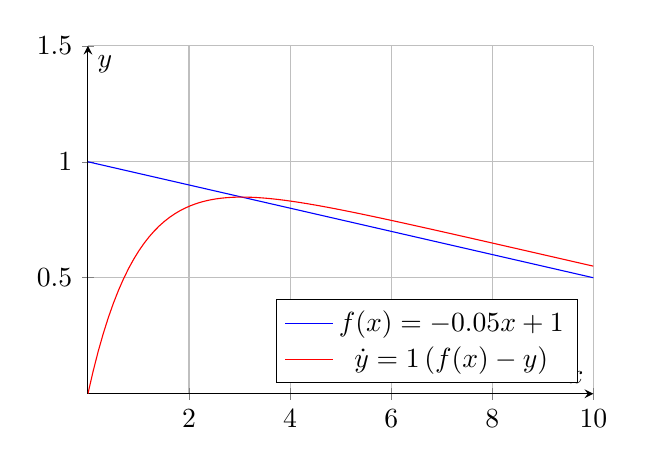
\begin{tikzpicture}
            \begin{axis}[axis lines=middle,xlabel=$x$,ylabel=$y$,grid=both,width=8cm,height=6cm,legend pos=south east,ymin=0,ymax=1.5]
                \pgfmathsetmacro{\aa}{-.05}
                \pgfmathsetmacro{\bb}{1}
                \pgfmathsetmacro{\cc}{1}
                \addplot[domain=0:10,samples=100,color=blue]{\aa*x+\bb};
                \addplot[domain=0:10,samples=100,color=red]{\aa*x+\bb+(\aa/\cc-\bb)*exp(-\cc*x)-\aa/\cc};
                \addlegendentry{$f(x)=\aa{}x+\bb$}
                \addlegendentry{$\dot{y}=\cc\left(f(x)-y\right)$}
            \end{axis}
        \end{tikzpicture}
        \caption{softening}
    \end{subfigure}\hfill
    \begin{subfigure}{0.48\textwidth}\centering
        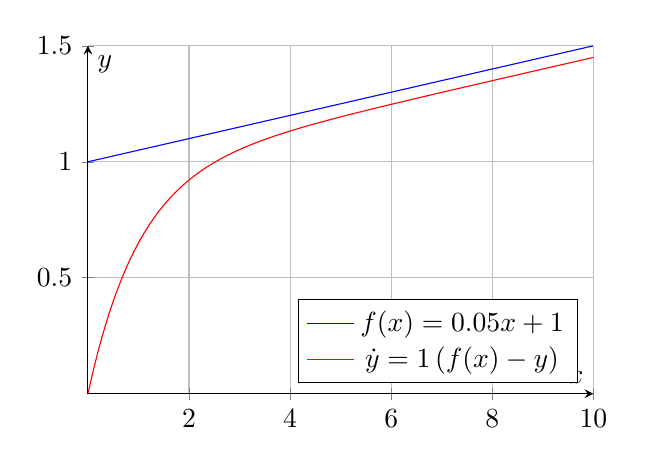
\begin{tikzpicture}
            \begin{axis}[axis lines=middle,xlabel=$x$,ylabel=$y$,grid=both,width=8cm,height=6cm,legend pos=south east,ymin=0,ymax=1.5]
                \pgfmathsetmacro{\aa}{0.05}
                \pgfmathsetmacro{\bb}{1}
                \pgfmathsetmacro{\cc}{1}
                \addplot[domain=0:10,samples=100,color=blue]{\aa*x+\bb};
                \addplot[domain=0:10,samples=100,color=red]{\aa*x+\bb+(\aa/\cc-\bb)*exp(-\cc*x)-\aa/\cc};
                \addlegendentry{$f(x)=\aa{}x+\bb$}
                \addlegendentry{$\dot{y}=\cc\left(f(x)-y\right)$}
            \end{axis}
        \end{tikzpicture}
        \caption{hardening}
    \end{subfigure}
    \caption{examples}\label{fig:examples}
\end{figure}
As can be seen from the figure, the solution may overshoot for softening bounds.
Furthermore, in both cases, the solution $y$ does \textbf{not} asymptotically approach the bound $f(x)$.
That is, the following condition does not hold for arbitrarily small $\epsilon$,
\begin{gather}
    \lim_{x\to\infty}\abs{y-f(x)}<\epsilon.
\end{gather}

To ensure that the solution is bounded by $f(x)$, let's consider the following function,
\begin{gather}
    y=f(x)\left(1-\exp\left(-bx\right)\right),
\end{gather}
since $1-\exp\left(-bx\right)\leqslant1$, it is guaranteed that $y\leqslant{}f(x)$.
The corresponding ODE can be derived as follows,
\begin{gather}\label{eq:strict_bound}
    y'=fb\exp\left(-bx\right)+f'\left(1-\exp\left(-bx\right)\right)=b\left(f-y\right)+\dfrac{f'}{f}y.
\end{gather}
After careful comparison, one could observe that \eqsref{eq:strict_bound} is in fact identical to the evolution rule presented in \eqsref{eq:original_core}.
\subsubsection{Revised Evolution Rule (Elastic Core)}
Based on the above observations, instead of defining an evolution rule for $\bc$ as shown in \eqsref{eq:original_core}, which turns out to be cumbersome when it comes to numerical implementation, one can apply the following decomposition,
\begin{gather}\label{eq:decomposition_core}
    \bc-\bbeta=F\bd,
\end{gather}
then the evolution of $\bc$ can be equivalently described by the evolution of $\bd$, which takes a very simple form,
\begin{gather}
    \dot{\bd}=c_e\left(z_e\bn-\bd\right)\gamma.
\end{gather}
Since $\bd$ defined in this manner is bounded by $z_e$, it is then guaranteed that $\bc-\bbeta\leqslant{}z_eF$.
\subsubsection{Revised Evolution Rule (Back Stress)}
Now since \eqsref{eq:decomposition_core} is adopted, it can also be applied to $\bbeta$ to allow its bound to evolve with the development of plasticity.
\begin{gather}\label{eq:decomposition_back}
    \bbeta=a^y\balpha,
\end{gather}
with $a^y=a^y\left(q\right)$ being the bound and $\balpha$ being the normalised back stress which shall have the following evolution rule.
\begin{gather}
    \dot{\balpha}=b\left(\bn-\balpha\right)\gamma,
\end{gather}
where $b$ is a constant that controls the evolution rate.
\subsection{A von Mises Material Model}
Within the von Mises framework, the shifted stress shall be computed as
\begin{gather}
    \beeta=\dev{\bsigma}-\left(\bbeta+\left(1-z\right)\left(\bc-\bbeta\right)\right),
\end{gather}
since now the new centre of the subloading surface is $\bbeta+\left(1-z\right)\left(\bc-\bbeta\right)$.
Account for \eqsref{eq:decomposition_core} and \eqsref{eq:decomposition_back}, the above expression can be rewritten as
\begin{gather}
    \beeta=\dev{\bsigma}-a^y\balpha+\left(z-1\right)\sigma^y\bd,
\end{gather}
where $\sigma^y=\sigma^y\left(q\right)$ denotes the yield stress that evolves with the accumulated plastic strain $q$.
\subsubsection{Subloading Surface}
The subloading surface shall be expressed as follows by replacing $F$ with $\sqrt{\dfrac{2}{3}}\sigma^y$.
\begin{gather}
    f_s=\norm{\beeta}-z\sqrt{\dfrac{2}{3}}\sigma^y.
\end{gather}
\subsubsection{Flow Rule}
Assuming associative plasticity, the flow rule is given by
\begin{gather}\label{eq:subloading_flow}
    \dot{\bvarepsilon^p}=\gamma\pdfrac{f_s}{\bsigma}=\gamma\dfrac{\beeta}{\norm{\beeta}}=\gamma\bn,
\end{gather}
where $\gamma$ denotes the plastic multiplier.
\subsubsection{Evolution Rules}
\paragraph{Accumulated Plastic Strain}
The accumulated plastic strain $q$ simply takes the accumulated magnitude of $\bvarepsilon^p$, thus, its rate form is
\begin{gather}
    \dot{q}=\sqrt{\dfrac{2}{3}}\norm{\dot{\bvarepsilon^p}}=\sqrt{\dfrac{2}{3}}\gamma.
\end{gather}
\paragraph{Isotropic Hardening}
The evolution of $\sigma^y$ depends on $q$, here we adopt general form that combines linear hardening and nonlinear saturation.
\begin{gather}
    \sigma^y=\sigma^i+k_\text{iso}q+\sigma^s_\text{iso}\left(1-e^{-m^s_\text{iso}q}\right),
    \end{gather}
    where $\sigma^i$ is the initial yield stress, $k_\text{iso}$ is the isotropic hardening modulus, $\sigma^s_\text{iso}$ is the saturation stress, and $m^s_\text{iso}$ is the saturation rate.
    \paragraph{Kinematic Hardening}
    The kinematic hardening bound $a^y$ takes a similar form,
    \begin{gather}
        a^y=a^i+k_\text{kin}q+a^s_\text{kin}\left(1-e^{-m^s_\text{kin}q}\right),
    \end{gather}
    where $a^i$ is the initial stress, $k_\text{kin}$ is the kinematic hardening modulus, $a^s_\text{kin}$ is the saturation stress, and $m^s_\text{kin}$ is the saturation rate.
    
    The normalised back stress $\balpha$ adopts an Armstrong--Frederick type evolution rule,
    \begin{gather}
        \dot{\balpha}=b\left(\sqrt{\dfrac{2}{3}}\bn-\balpha\right)\gamma.
    \end{gather}
    \paragraph{Elastic Core}
    \begin{gather}
    \dot{\bd}=c_e\left(\sqrt{\dfrac{2}{3}}z_e\bn-\bd\right)\gamma.
\end{gather}
\subsection{Numerical Implementation}
\subsubsection{Some Simplifications}
Noting that $\dot{\balpha}$ is a linear function of $\balpha$, taking advantage of the implicit Euler method, one could express $\balpha$ in its explicit form.
\begin{gather}
    \balpha_n+b\left(\sqrt{\dfrac{2}{3}}\bn-\balpha\right)\gamma=\balpha\qquad\rightarrow\qquad
    \balpha=\dfrac{\gamma\sqrt{\dfrac{2}{3}}b\bn+\balpha_n}{1+\gamma{}b}.
    \end{gather}
    Similarly, $\bd$ can be expressed as
    \begin{gather}
        \bd_n+c_e\left(\sqrt{\dfrac{2}{3}}z_e\bn-\bd\right)\gamma=\bd\qquad\rightarrow\qquad\bd=\dfrac{\gamma{}\sqrt{\dfrac{2}{3}}c_ez_e\bn+\bd_n}{1+\gamma{}c_e}.
    \end{gather}
    On the other hand, the deviatoric stress $\bs$ shall be computed via the trial stress $\bsigma^\text{trial}$,
    \begin{gather}
    \bs=\dev{\bsigma}=\dev{\bsigma^\text{trial}-\gamma2G\bn}=\dev{\bsigma^\text{trial}}-\gamma2G\bn=\bs^\text{trial}-\gamma2G\bn.
\end{gather}

The shifted stress $\beeta$ is then
\begin{gather}
    \begin{split}
        \beeta & =\bs-a^y\balpha+\left(z-1\right)\sigma^y\bd                                                                                                                                                \\
               & =\bs^\text{trial}-\gamma2G\bn-a^y\dfrac{\gamma{}\sqrt{\dfrac{2}{3}}b\bn+\balpha_n}{1+\gamma{}b}+\left(z-1\right)\sigma^y\dfrac{\gamma{}\sqrt{\dfrac{2}{3}}c_ez_e\bn+\bd_n}{1+\gamma{}c_e}.
    \end{split}
\end{gather}
Rearranging gives
\begin{multline}
    \beeta+\gamma2G\bn+\sqrt{\dfrac{2}{3}}b\dfrac{\gamma{}a^y}{1+\gamma{}b}\bn+\sqrt{\dfrac{2}{3}}c_ez_e\left(1-z\right)\dfrac{\gamma{}\sigma^y}{1+\gamma{}c_e}\bn=\\\bs^\text{trial}-\dfrac{a^y}{1+\gamma{}b}\balpha_n+\left(z-1\right)\dfrac{\sigma^y}{1+\gamma{}c_e}\bd_n.
\end{multline}
One could denote
\begin{gather}\label{eq:zeta}
    \bzeta=\bs^\text{trial}-\dfrac{a^y}{1+\gamma{}b}\balpha_n+\left(z-1\right)\dfrac{\sigma^y}{1+\gamma{}c_e}\bd_n,
\end{gather}
such that
\begin{gather}
        \left(\norm{\beeta}+\gamma2G+\sqrt{\dfrac{2}{3}}b\dfrac{\gamma{}a^y}{1+\gamma{}b}+\sqrt{\dfrac{2}{3}}c_ez_e\left(1-z\right)\dfrac{\gamma{}\sigma^y}{1+\gamma{}c_e}\right)\bn=\bzeta.
        \end{gather}
    It can be noted that each term in the bracket is non-negative by definition, thus it is correct to conclude that
    \begin{gather}\label{eq:zeta_norm}
    \norm{\beeta}+\gamma2G+\sqrt{\dfrac{2}{3}}b\dfrac{\gamma{}a^y}{1+\gamma{}b}+\sqrt{\dfrac{2}{3}}c_ez_e\left(1-z\right)\dfrac{\gamma{}\sigma^y}{1+\gamma{}c_e}=\norm{\bzeta},
\end{gather}
and
\begin{gather}
    \bn=\dfrac{\beeta}{\norm{\beeta}}=\dfrac{\bzeta}{\norm{\bzeta}}.
\end{gather}
Although it is not possible to simplify more, one shall realise that $\bzeta$ is a function of $\bvarepsilon$, $\gamma$ and $z$ only.
Its derivatives can be computed as follows.
\begin{gather}
    \pdfrac{\bzeta}{\gamma}=-\dfrac{\ddfrac{a^y}{\gamma}\left(1+\gamma{}b\right)-ba^y}{\left(1+\gamma{}b\right)^2}\balpha_n+\left(z-1\right)\dfrac{\ddfrac{\sigma^y}{\gamma}\left(1+\gamma{}c_e\right)-c_e\sigma^y}{\left(1+\gamma{}c_e\right)^2}\bd_n,\\
    \pdfrac{\bzeta}{z}=\dfrac{\sigma^y}{1+\gamma{}c_e}\bd_n,\\
    \pdfrac{\bzeta}{\bvarepsilon}=2G\mathbb{I}_\text{dev}.
\end{gather}
\subsubsection{Local System}
The local system consists of two residuals, $f_s$ and $z$.
\begin{gather}
    \mb{R}=\left\{
    \begin{array}{l}
        \norm{\beeta}-\sqrt{\dfrac{2}{3}}z\sigma^y, \\[2mm]
        z-z_n-\sqrt{\dfrac{2}{3}}U\gamma.
    \end{array}
    \right.
\end{gather}
Taking the local variable as $\mb{x}=\begin{bmatrix}
        \gamma & z
    \end{bmatrix}^\mT$, the Jacobian $\mb{J}$ shall be written as
\begin{gather}
    \mb{J}=\begin{bmatrix}
        \pdfrac{\norm{\beeta}}{\gamma}-\sqrt{\dfrac{2}{3}}z\ddfrac{\sigma^y}{\gamma} & \pdfrac{\norm{\beeta}}{z}-\sqrt{\dfrac{2}{3}}\sigma^y \\[4mm]
        -\sqrt{\dfrac{2}{3}}U                                                        & 1-\sqrt{\dfrac{2}{3}}\gamma{}\ddfrac{U}{z}
    \end{bmatrix}.
\end{gather}
It is possible to avoid cumbersome computation of derivatives of $\norm{\beeta}$ by taking advantage of \eqsref{eq:zeta_norm}.
By noting that the derivatives of $\norm{\bzeta}$ can be further expanded as
\begin{gather}
    \pdfrac{\norm{\bzeta}}{}=\bn:\pdfrac{\bzeta}{},
\end{gather}
then
\begin{gather}
    \pdfrac{\norm{\beeta}}{\gamma}=\bn:\pdfrac{\bzeta}{\gamma}-2G-\pdfrac{}{\gamma}\left(\sqrt{\dfrac{2}{3}}b\dfrac{\gamma{}a^y}{1+\gamma{}b}+\sqrt{\dfrac{2}{3}}c_ez_e\left(1-z\right)\dfrac{\gamma{}\sigma^y}{1+\gamma{}c_e}\right),\\
    \pdfrac{\norm{\beeta}}{z}=\bn:\pdfrac{\bzeta}{z}+\sqrt{\dfrac{2}{3}}c_ez_e\dfrac{\gamma{}\sigma^y}{1+\gamma{}c_e}.
\end{gather}
\subsubsection{Consistent Tangent Operator}
It is possible to differentiate the local equilibrium $\mb{R}=\mb{0}$ to obtain
\begin{gather}
    \pdfrac{\mb{R}}{\bvarepsilon}+\pdfrac{\mb{R}}{\mb{x}}\ddfrac{\mb{x}}{\bvarepsilon}=\mb{0}.
\end{gather}
This gives
\begin{gather}\label{eq:local_equilibrium}
    \ddfrac{\mb{x}}{\bvarepsilon}=-\left(\pdfrac{\mb{R}}{\mb{x}}\right)^{-1}\pdfrac{\mb{R}}{\bvarepsilon}=-\mb{J}^{-1}\pdfrac{\mb{R}}{\bvarepsilon}.
\end{gather}
Noting that
\begin{gather}
    \pdfrac{\norm{\beeta}}{\bvarepsilon}=\bn:\pdfrac{\bzeta}{\bvarepsilon}=2G\bn:\mathbb{I}_\text{dev}=2G\bn,
\end{gather}
then in the matrix form,
\begin{gather}
    \pdfrac{\mb{R}}{\bvarepsilon}=2G\begin{bmatrix}
        \bn^\mT \\\mb{0}
    \end{bmatrix}.
\end{gather}
By solving \eqsref{eq:local_equilibrium}, one could obtain $\ddfrac{\mb{x}}{\bvarepsilon}$, we are interested in the first row, which can be explicitly written as
\begin{gather}
    \ddfrac{\gamma}{\bvarepsilon}=-2G\dfrac{1-\sqrt{\dfrac{2}{3}}\gamma{}\ddfrac{U}{z}}{\det\mb{J}}\bn^\mT.
\end{gather}
Now from the stress update expression, it is possible to derive the consistent tangent operator as
\begin{gather}
    \ddfrac{\bsigma}{\bvarepsilon}=\mb{D}-2G\left(\pdfrac{\bn}{\bvarepsilon}\gamma+\bn\ddfrac{\gamma}{\bvarepsilon}\right).
\end{gather}
In the meantime, by $\bn=\dfrac{\bzeta}{\norm{\bzeta}}$, the derivative of $\bn$ with respect to $\bvarepsilon$ can be shown as
\begin{gather}
    \pdfrac{\bn}{\bvarepsilon}=\dfrac{2G}{\norm{\bzeta}}\left(\mathbb{I}_\text{dev}-\bn\bn^\mT\right),
\end{gather}
after some algebra, the consistent tangent operator can be written as
\begin{gather}
    \ddfrac{\bsigma}{\bvarepsilon}=\mb{D}-\dfrac{4G^2\gamma}{\norm{\bzeta}}\mathbb{I}_\text{dev}+4G^2\left(\dfrac{\gamma}{\norm{\bzeta}}+\dfrac{1-\sqrt{\dfrac{2}{3}}\gamma{}\ddfrac{U}{z}}{\det\mb{J}}\right)\bn\bn^\mT.
\end{gather}
\subsubsection{Remarks}
Compared to the previous implementation, the formulation proposed in this work dramatically reduces the size of local system from \num{20} to \num{2}.
We also present the explicit expression of the consistent tangent operator.